%included in thesis.tex,



\chapter{Background and Literature Study}
\label{chap2}
This chapter will try to outline the basics needed to understand this report. Mathematical
knowledge are crucial to understand the principles used in robot navigation and decision
making. The topics treated here include, general reference frames, homogeneous coordinate
representations, camera modeling, feature matching, map representations and optimization
criteria.



\section{Basics}

\subsection{Reference Frames}
	Movement must be described relative to something. This is the task of the reference systems. There are
	4 important reference system. The ECI (Earth Centre Inertial) which is a truly inertial reference
	frame, i.e. it is not accelerating. Its axis are pointing through the north pole and through the
	equatorial line of the Earth, fixed toward stationary points in space. The centre is as the name
	suggests in the centre of the Earth. 
	
	ECEF (Earth-Centre Earth-Fixed) is another reference frame. It is defined same as the ECI coordinate
	system, but the axis are rotating with the same rate as the Earths rotation rate. This means that this frame
	is not
	strictly inertial, but the angular velocity of the Earths rotation are considered very small, and can
	be neglected compared to other velocities in the same frame. Position on the earth are described by
	\emph{longitude} and \emph{latitude}.

	An important reference frame when considering local motion are the NED (North East Down) frame. This
	frame is defined as the tangent plane on the current position, and moving with the object. The axis
	are pointing towards north, east and down. This frame can be used in local, and small areas, but are
	not valid for intercontinental travel. This frame will primarily be used in this report. 

	The last but important frame are the Body frame, which is the local frame of the object of interest.
	The body frame are defined as the x-axis along its forward movement, y-axis to the right of the
	movement direction, and the last pointing downward, to complete the right-hand system. The
	origin are defined in the Centre of Gravity of the object. This frame are convenient when
	defining velocities, forces and moments. More on reference frames in \cite{fossen} and
    \cite{forsell}.

    The reference frames that will be considered in this report are the \emph{NED}- and
    \emph{body} frames. In addition to these two frames there are the last, but not least
    important frame, called the \emph{single-sensor} frame. This is where the output from
    the sensors are defined. These output need to be transformed into the \emph{body} and
    to the \emph{NED} frame to make sense for the control system and ultimately for the
    user. 

    The \emph{single-sensor} frames are where the individual sensors give readings. The
    exact mount point relative to the centre-of-gravity need to be defined, to make the
    transformation to other frames possible. The domain of the \emph{single-sensor} frames
    are defined in accordance to the domain of the sensor, i.e. the domain of a Laser
    Range Finder, which gives angles and ranges in the plane are two dimensional. 


\subsection{Homogeneous Transformation Coordinates}
To represent transformations, i.e. rotations, translations, shear and scaling, it is
practical to represent those transformations in matrix form. But it is not mathematically
possible to represent both rotations and translations in the same matrix as long as it is
contained in $\mathbb{R}^3$. 

To overcome this problem, the coordinates are projected into a fourth dimensional space.
All points and vectors gain an extra element which describes if the coordinate is a vector
or a point. 
\begin{equation}
        \mathbf{v} = \left[ \begin{array}{c}
                                    x_v \\
                                    y_v \\
                                    z_v \\
                                    w_v  \end{array} \right]  =
                     \left[ \begin{array}{c}
                                    1 \\
                                    0 \\
                                    0 \\
                                    0  \end{array} \right] \quad \quad
        \mathbf{p} = \left[ \begin{array}{c}
                                    x_p \\
                                    y_p \\
                                    z_p \\
                                    w_p  \end{array} \right]  =
                     \left[ \begin{array}{c}
                                    1 \\
                                    0 \\
                                    0 \\
                                    1  \end{array} \right] \quad \quad
\end{equation}
Here $\mathbf{v}$ is a vector with the fourth element as zero, while $\mathbf{p}$ is a
point with the fourth element equal one.

This leads us to the \emph{Transformation Matrix} which is a $4 \times 4$ matrix. For
example a matrix representing rotation and translation will look like this
\begin{equation}
    \label{chap2:eq-TransformationMatrix}
    \mathbf{T_{rt}} = \left [ \begin{array}{cccc}
                                r_{xx} & r_{xy} & r_{xz} & t_x \\
                                r_{yx} & r_{yy} & r_{yz} & t_y \\
                                r_{zx} & r_{zy} & r_{zz} & t_z \\
                                0  & 0  & 0  & 1  \end{array} \right]
\end{equation}
Here the $r_{ii}$ coefficients are rotation parameters and the $t_i$ coefficients are the
translation parameters. The rotation coefficients are calculated from the Euler angles.

Likewise, scaling might be performed by the following transformation matrix
\begin{equation}
    \label{chap2:eq-TransformationMatrixScaling}
    \mathbf{T_S} = \left [ \begin{array}{cccc}
                                S_x & 0 & 0 & 0 \\
                                0 & S_y & 0 & 0 \\
                                0 & 0 & S_z & 0 \\
                                0 & 0 & 0 & 1 
                                 \end{array} \right]
\end{equation}
All of this transformations might be combined into a single matrix by multiplying the
matrices together, in the reverse of the order of which the transformations are carried
out. 


\section{Ranging Techniques}
The measure of distances and ranges are important and there are various ways of doing
this. Most techniques include the measure of time-of-flight of some signal and calculating
the distance from the known travel velocity of the signal. This requires the signal
emitted to be reflected, captured and processed at or close to the emitter. The signal is
usually electromagnetic or sound based, which allows for different kinds of modulations to
make the signal easier to recognize at the receiver.


This section will first outline the usual range determination techniques then go into the
more specific sensor characteristics in later sections.


\subsection{Triangulation}
\begin{figure}[htbp]
    \centering
    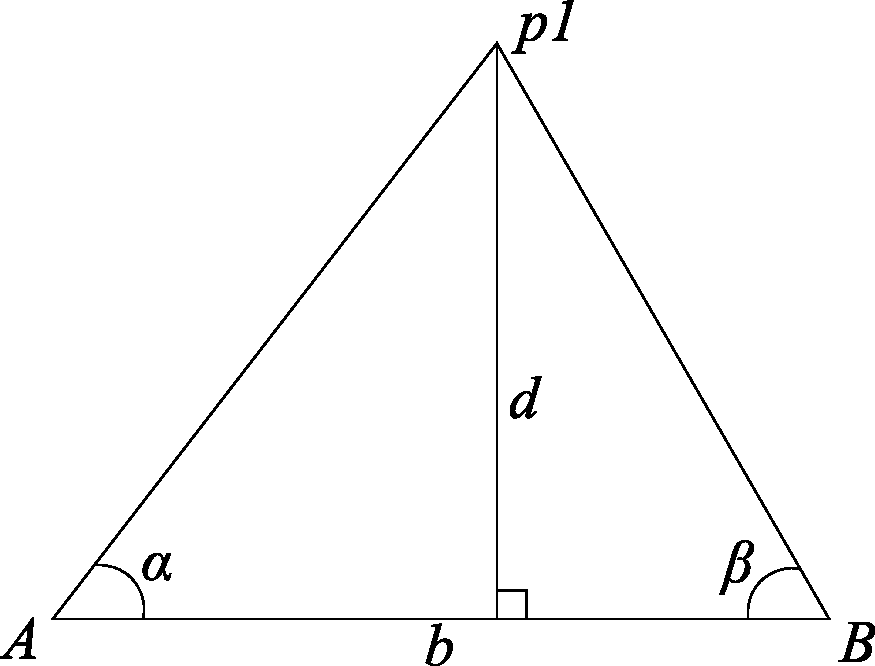
\includegraphics[width=0.55\textwidth]{pics/triangulation}
    \caption{Triangulation setup}
    \label{chap2:fig-triangulation}
\end{figure}
The technique of triangulation is an old and well-known technique for range determination.
Two points with known locations are used. The distance between the two points, $A$ and $B $are called
the \emph{baseline}. Instead of measuring the range to $p1$ directly, the angles
from $A$ and $B$ and the baseline is used to calculate the range to the third point, $p1$,
according to Equation \ref{chap2:eq-triangulation}. See Figure
\ref{chap2:fig-triangulation}.
\begin{equation}
    \label{chap2:eq-triangulation}
    d = b \frac{\sin{\alpha} \sin{\beta}}{\sin{\alpha + \beta}}
\end{equation}
This technique is accurate for as long as all the points are in the same plane.


\subsection{Time-of-Flight Measurement}
This method of range determination is the most common, and utilizes the travel time of the
emitted signal. The signal might be in light, radio or sound waves. The precision of the
range greatly depend on the type of signal, the medium which it travels and the quality of
the time-measuring device. By knowing the velocity of the emitted signal and assuming it
is constant, the distance it travels can be determined with great accuracy according to 
Equation \eqref{chap2:eq-tof}
\begin{equation}
    \label{chap2:eq-tof}
    d = v \frac{t}{2}
\end{equation}



\section{Various Sensors Used in Robotics}
This section concerns the use of different kind of sensors in robotic applications. Only
sensors which are compliant to the overall perspective will be dealt with. This includes
laser range finders, ultrasound and Sonar sensors, Time-of-Flight cameras and
stereo cameras. 


\subsection{1D Sensors}

\subsubsection{Proximity Sensors}
Proximity senors are used to detect if a object is near or not. These sensors are usually
small and not very expensive. This means that a number of these can be fit on a robot
without impacting either price, size or weight of the robot. 

Proximity sensors usually consists of a source and a detector. The detector detects the
signal from the source only if an object is close enough, and thereby triggering the
output of the sensor. The medium used depends on the application, and can be everything
from sound, light or electromagnetic waves. 
\cite{proximity}

\subsection{2D Sensors}

\subsubsection{Laser Range Finders}
When looking at Laser Range Finder, there are 3 techniques for determining the distance,
\emph{optical triangulation}, \emph{pulse Time-of-Flight} and \emph{frequency modulated
continuous wave} (FMCW). \cite{laser-ranging-critical-review}

\paragraph{Optical Triangulation}
Optical is very similar to triangulation described above and uses the same principle.
A light source are placed at the one end of the
baseline, and a light sensor at the other end which senses the reflected light from the
light source. The principle is basically the same as in normal triangulation. But, due to
the fact that a light source is used, and more closely a laser light source, the surface
that the laser light hits, the dot detected by the photo detector at the other end of the
baseline, needs to ''stay in focus``. If this is not done the laser dot will become a
blurred disc and the uncertainty to the point will become larger. To force the dot to
always be in focus, a special aligning of the lenses and photo detector are used, called 
the \emph{Scheimpflug} condition. The interested reader are referred to
\cite{laser-ranging-critical-review}.

The laser dot is contaminated with speckle noise which makes it more difficult to find the
exact center of the projected dot. This makes the determination of the along the third
dimension a bit more tricky, because of the positional uncertainty introduced by the
noise. Frequency of the light, angle and area of the collecting lenses and photo detector
are parameters that influence the position uncertainty. 

This technique can be used for pipeline profiling, i.e. Assessing the quality of the pipe
and finding damages, weak spots, corrosion, and other things worth noting when doing a pipe
inspection. \cite{optical-pipe-inspection} describes an instrument for recording sizes and
internal structure of almost any pipe size, using an optical triangulation scheme mounted
on a rotating head. 


\paragraph{Pulsed Time-of-Flight}
\label{chap2:subsec-lrf}
The technique referred to as pulsed time-of-flight refers to the time taken of a pulse
train of laser light to be reflected back to the emitter. Light travels around 30 cm/ns,
this means that to get 1 mm accuracy the accuracy of the timing devices should be
6.7 ps.

Only a single laser pulse is necessary for the determination of the range with centimeter
precision this technique is suitable for fast measurements and range sweeps. If the
measurements are averaged millimeter precision might be acquired. 

The application and ranges that are going to be measured are dependant on what kind of
laser which is selected. The energy in the laser pulse effects the amplitude of the
reflected light and in turn affects the measurement accuracy.

Major sources of inaccuracies in a pulsed time-of-flight range finders are timing jitter,
nonlinearities, walk and drift. Jitter in timing is the source of precision errors in the
system. Precision also deteriorates as the distance increase and the reflected pulse
amplitude decrease proportional to the square of the distance\cite{pulsed-tof}.
Walk errors are due to shape variations in the pulse, which will create errors in the
timing measurement. 





\paragraph{Frequency Modulated Continuous Wave}
This technique have been used in in applications such as, surface profiling, tomography
reflectography and positioning. This is a technique which have large dynamic range and
high resolution at short range sensing. The principle is that a laser diode is applied
with a frequency periodically shifted by $\Delta f$. The signal is usually done with
applying a saw-tooth biased current to a wavelength-tunable laser diode. This saw-tooth
signal is also sent to be mixed with the reflected signal. The phase difference in the
reference signal and the reflected signal is $\tau = 2 R / c$ where $R$ is the range of
the traveled signal. The range is proportional to the intermediate frequency, i.e. the
frequency difference due to the travel time
\begin{equation}
    f_i = \Delta f \tau /t_m = 2 \Delta f R /c t_m
\end{equation}
$t_m$ is the ramp period of the saw-tooth signal. 

Both $\tau$ and $f_i$ can be measured, which one that is measured depends on the required
range and resolution. If the intermediate frequency is measured the resolution is best,
since the ramp time can be chosen freely, the need for high speed electronics are not
necessary, and a simple frequency counter in the kilohertz domain can be used to give the
sensor millimeter resolution.

Limitations of this technique is that the frequency characteristics of the laser diode is
seldom linear, which will result in a nonlinear reference signal, which leads to
variations in the intermediate frequency measurement.
\cite{laser-ranging-critical-review}.

\subsubsection{Sonar}
Sonars utilize sound waves for determining distance. It uses the time-of-flight principle
to measure the distance, assuming that the velocity of the sound wave can be determined
within some accurate bounds. The problem is that the travel time of sound varies with a
number of parameters limiting the accuracy of the range estimate substantially. 

There are a number of different sonar techniques. The most common are the narrow beam
sonars, which scans the environments like the 2D Laser Range Finders. \cite{mathisen}

Using sound as a carrier in air is usually not preferred, because the sound waves travels
much slower in air, and is quickly attenuated. This sensor type will not be considered for
the application in question. 


\subsection{3D Sensors}

\subsubsection{Stereo Vision}
Stereo vision is an inexpensive way of finding range measurements. The setup is two or
more cameras some distance away from each other. This distance is called the
\emph{baseline}. The camera images are then compared and a common reference point is
found. The difference between the images are then used together with the baseline distance
to triangulate the common reference point and then find the distance to the observed
object. 

The process of Stereo Imaging involves 4 steps when using two cameras \cite{openCV}:
\begin{enumerate}
    \item Remove radial and tangential lens distortion caused by inexpensive lenses and
        image chips. This outputs \emph{undistorted} images. 
    \item \emph{Rectify} the images. This adjusts the angles and distances between the cameras.
        This outputs row-aligned images.
    \item Find the same features in the left and right camera view. This process is called
        finding \emph{stereo correspondences}. This outputs a \emph{disparity} map, which
        is the difference in x-coordinate of the feature in the left and the right image. 
    \item If the geometric configuration of the cameras are known, the disparity map can
        be translated into depth map with the help of \emph{triangulation}. This final
        step is called \emph{reprojection}.
\end{enumerate}
This steps will be described in detail below. 


\paragraph{Pinhole Camera Model}
A camera model is needed to understand how light is captured on the image plane. To do
this a \emph{pinhole camera} model is used to capture light form a point. This model
assumes that only one light ray from each point travels trough a infinite small hole in
a plane, called the \emph{focal} plane and hits a second plane, called \emph{image} plane.
These two planes are placed a distance, $f$ from each other. Using elemental geometry the
coordinates of the real world point imaged at the image plane can be calculated. 
\begin{equation}
    -x_i = f \frac{X}{Z}
\end{equation}
where
\begin{equation}
    P_i = \left [ \begin{array}{c}
        x_i \\
        y_i 
    \end{array} \right]  \in \mathbb{R}^2 \quad \quad P_w = \left [
    \begin{array}{c}
        X \\
        Y \\
        Z \\ 
    \end{array} \right] \in \mathbb{R}^3 
\end{equation}
\begin{figure}[hbtp]
    \centering
    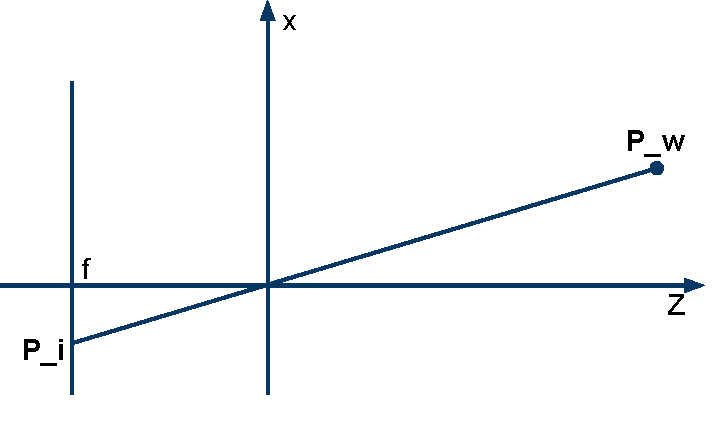
\includegraphics[width=0.7\textwidth]{pics/pinhole_model}
    \caption{Pinhole Camera Model showing two dimensions}
    \label{chap2:fig-pinholemodel}
\end{figure}

Figure \ref{chap2:fig-pinholemodel} shows the configuration with the pinhole located at
Origo and the image plane located at $f$. Where the pinhole is are often termed
\emph{center of projection}. The x axis of the image is located
upwards, while the real Z axis are the horizontal axis, that are called the
\emph{optcal axis} or the \emph{principal axis}. This lead us to the next parameters which need to be defined.

The optical axis should ideally always be aligned with the center of projection. Due to
manufacturing inaccuracies this is rarely the case, therefor we need two more parameters
in to complete the pinhole model equations. This parameters are $c_x$ and $c_y$ which
describes the offset of the optical axis from the center of projection. Also the need for
different focal lengths in $x$ and $y$ might also be a necessity, because the individual
pixels on a typical low-cost image chip is rectangular rather than square. Now the
equations relating real-world coordinates to image coordinates can be written.
\cite{openCV}
\begin{equation}
    x_i = f_x \frac{X}{Z} + c_x \quad \quad y_i = f_y \frac{Y}{Z} + c_y
\end{equation}

The equations above are the \emph{projective} transformations, and are convenient to
write using homogeneous coordinates and arrange the parameters into a single $3\times 3$
matrix. This matrix is sometimes called the \emph{camera intrinsic} matrix. 

\paragraph{Lens Distortion}
\label{chap2:sec-distortion}
Because very little light goes through the pinhole, and to make the camera practical for
real world use, lenses are used to bend, i.e. focus more light to the projective plane.
This allows for faster imaging of the world, but is also the source of more distortions
and inaccuracies. 

There are two types of lens distortions, \emph{radial} and \emph{tangential}. Radial
distortions are due to the lens construction. Most distortion occurs towards the edges of
the lens. This can be seen in pictures as ``barrel'' or ``fish-eye'' effects. These
effects are more present in cheap cameras which does not have the fancy lenses and optics
that the more high-end cameras have. There is also other types of distortions in imaging
systems, but they have typical lesser effects on the images, and will not be taken into
account. 

To model radial lens distortions the approach described by Brown in
\cite{lens-calibration} are used. The radial distortion are in practice small and can be
described by the two first terms of a Taylor series expansion around the center of the
lens. If the lens have high radial distortion, like fish-eye lenses a third term are
appended. The radial location of the point on the image plane can in general be described
like the equations below. 
\begin{equation}
\begin{aligned}
    x_{corrected} &= x_i ( 1 + k_1 r^2 + k_2 r^4 + k_3 r^6 ) \\
    y_{corrected} &= y_i ( 1 + k_1 r^2 + k_2 r^4 + k_3 r^6 ) 
\end{aligned}
\end{equation}

Tangential distortion is due to manufacturing defects which causes the lens not to be
perfectly parallel to the imaging plane. This causes the image to become more like a
trapezoid. This can be modeled by equations \eqref{chap2:eq-tangential-distortion}. The
derivation of this equations can be found in \cite{brown66}.
\begin{equation}
    \label{chap2:eq-tangential-distortion}
    \begin{aligned}
        x_{corrected} &= x_i + (2 p_1 y_i + p_2 (r^2 + 2 x_i^2)) \\
        y_{corrected} &= y_i + ( p_1 (r^2 + 2 y_i^2) + 2 p_2 x_i))
    \end{aligned}
\end{equation}
The parameters $p_1$ and $p_2$ are the tangential distortion parameters. This parameters
gives enough information about the lens and camera to make corrections to the picture and
make the matching method easier and the measurements more accurate. This calibrations will
be shown in Chapter \ref{chap3-sensors} for the selected stereo cameras. 

\begin{figure}[htbp]
    \centering
    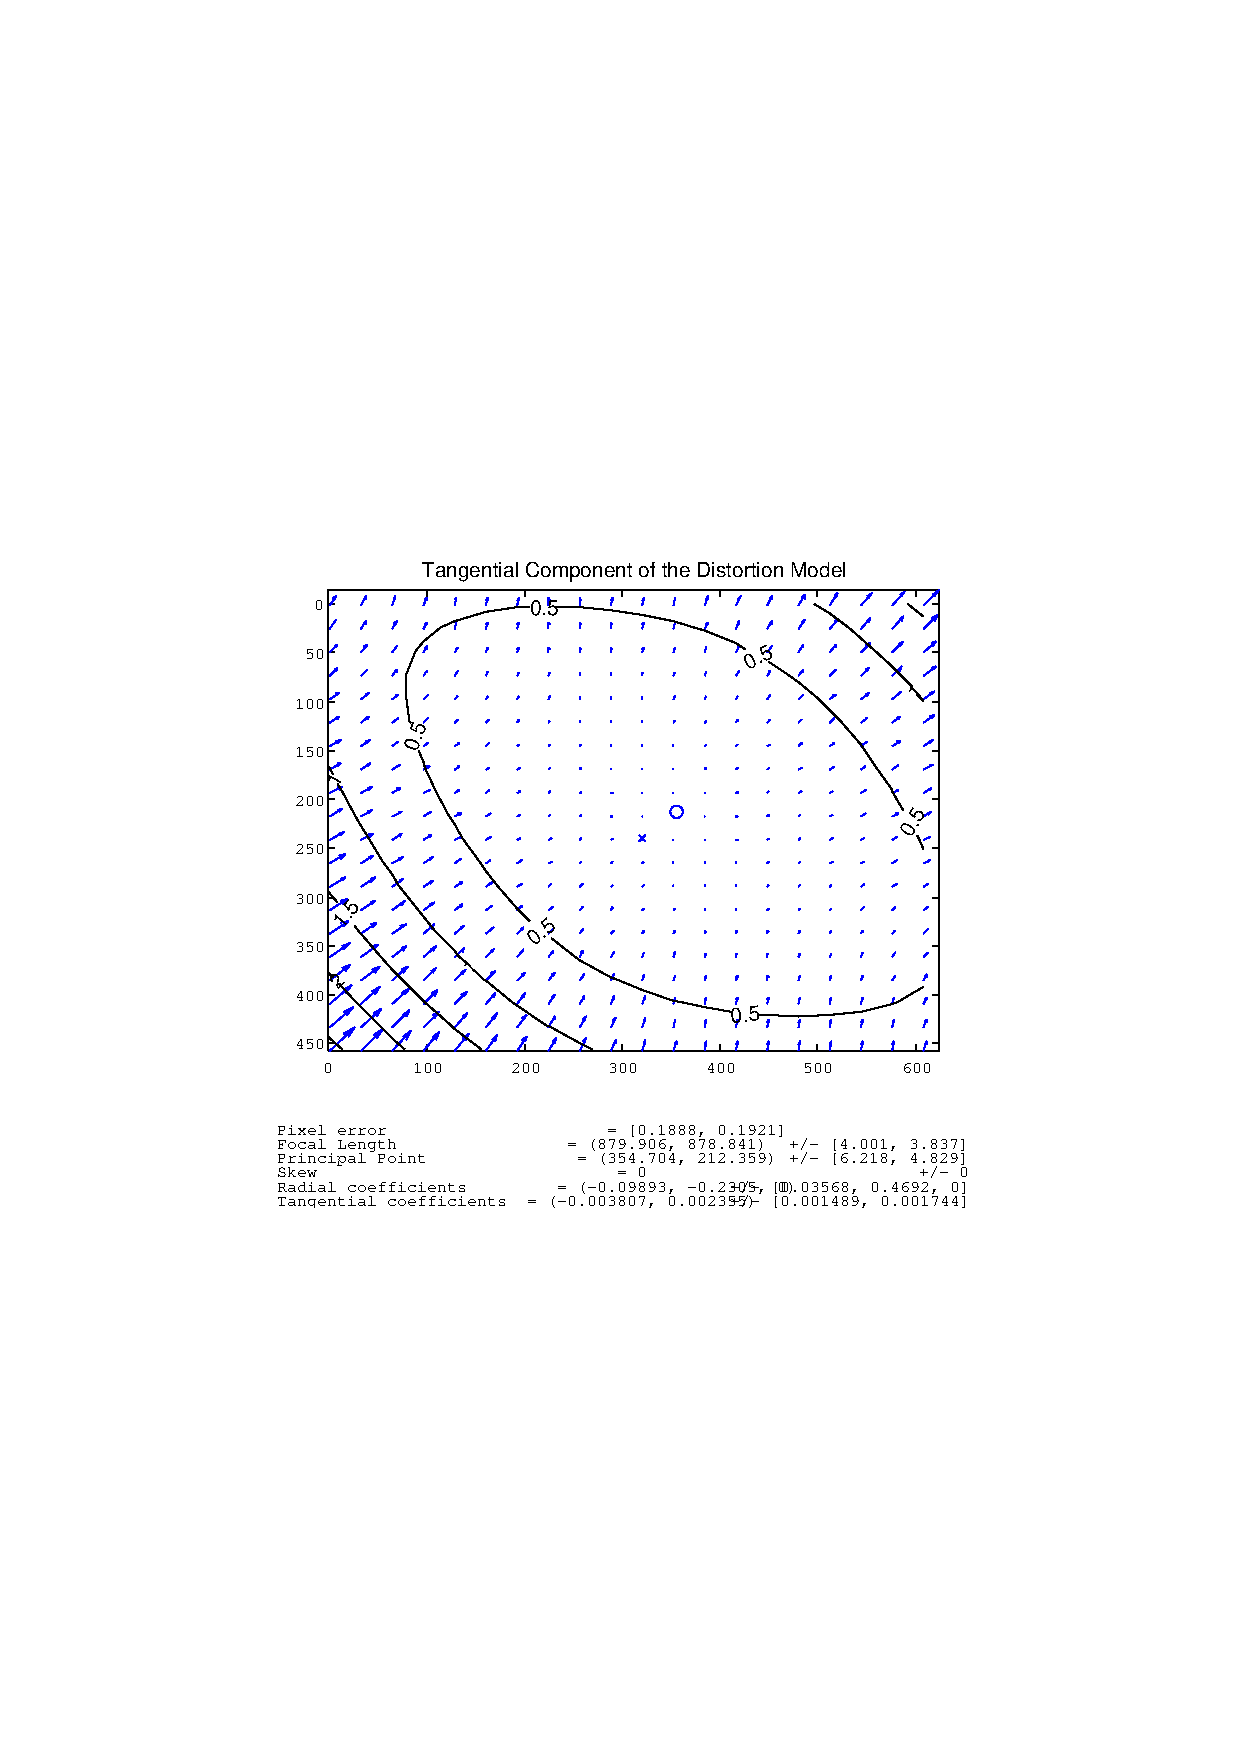
\includegraphics[width=0.45\textwidth]{pics/left_tang_dist}
    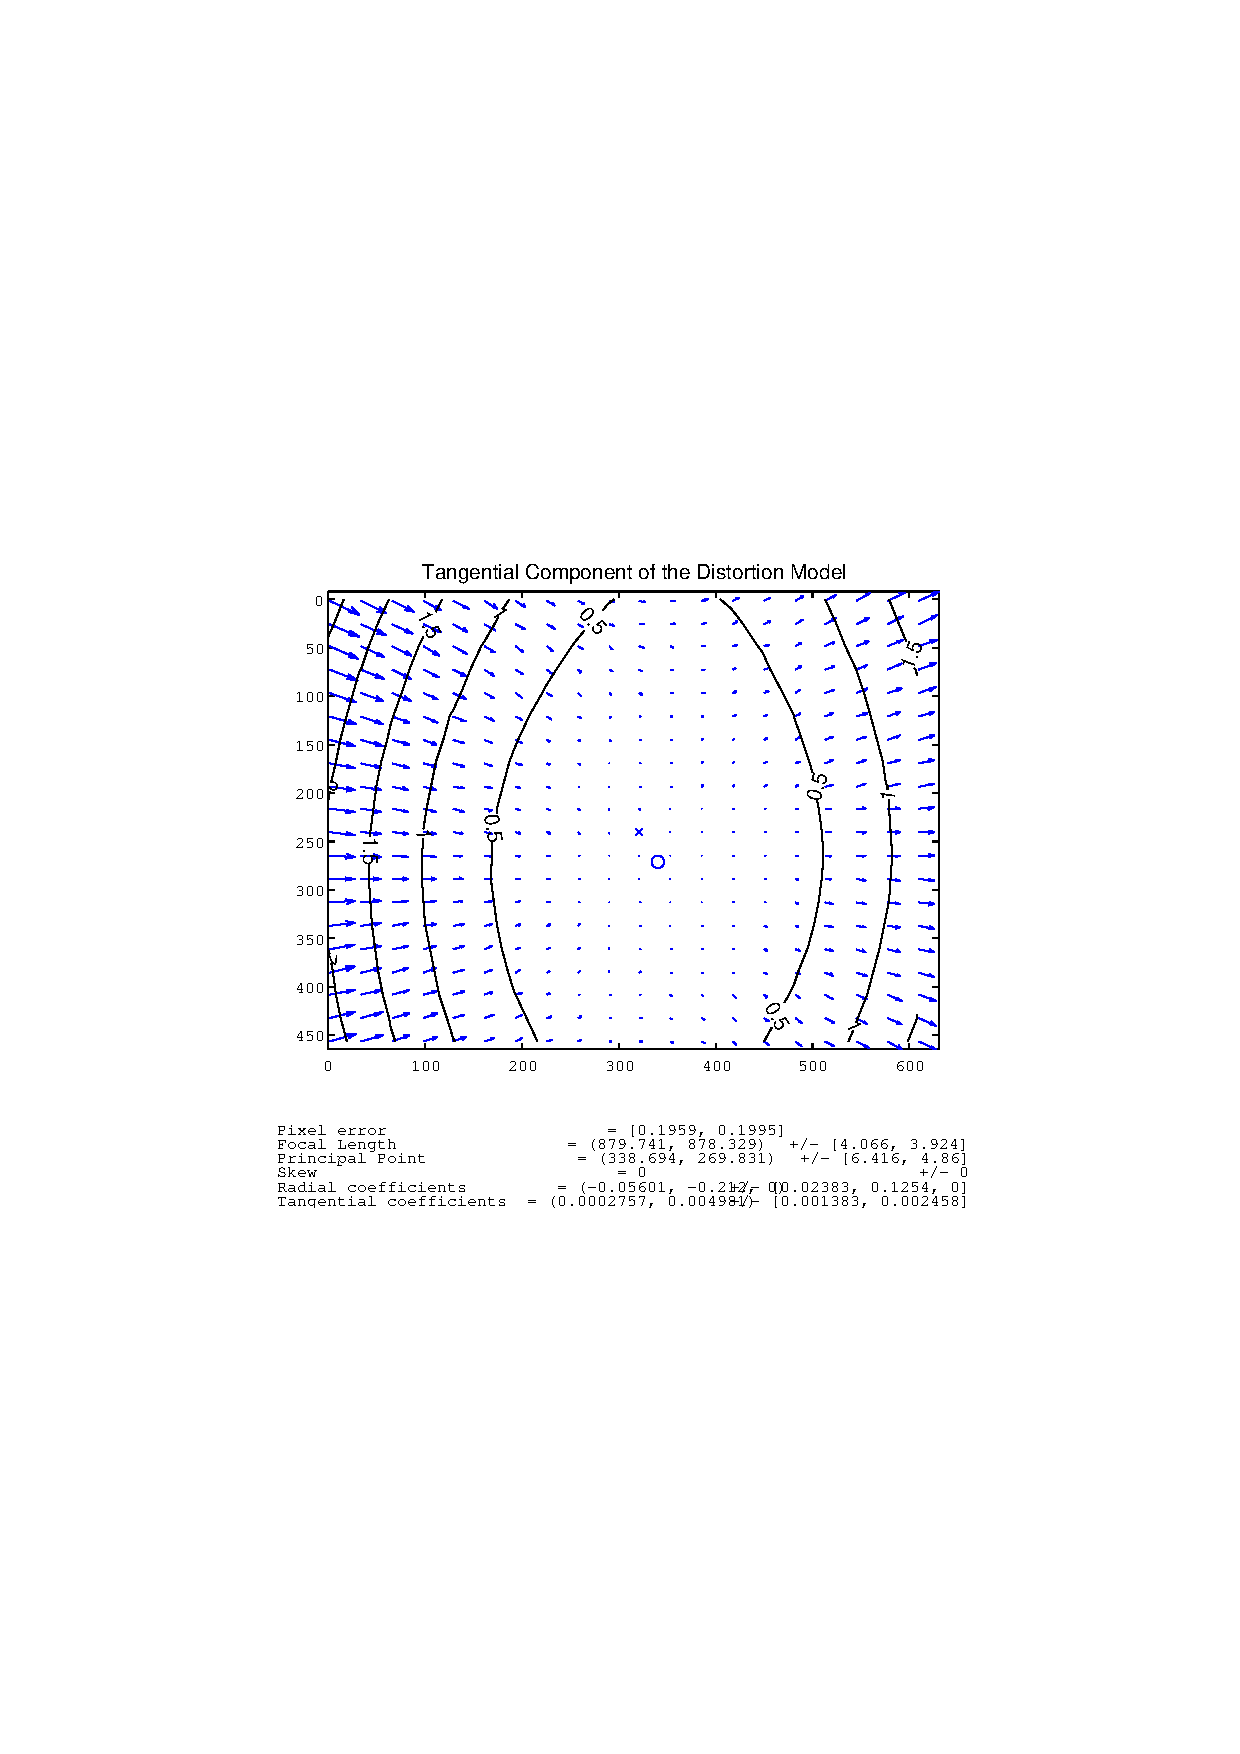
\includegraphics[width=0.45\textwidth]{pics/right_tang_dist}
    \caption{The tangential distortion for the left and right camera of the Minoru 3D
    webcam}
    \label{chap2:fig-tang-dist}
\end{figure}
Figure \ref{chap2:fig-tang-dist} show a plot for the left and right camera of the stereo
rig. As seen from the figure, the cameras are supposed to be identical, but the tangential
distortion can be very different, and clearly show the need to estimate and rectify the
images. 


\paragraph{Epipolar Geometry}
To describe the stereo rig and geometry between the left and right cameras, the term
\emph{epipolar geometry} is introduced. Epipolar geometry exists between any two cameras.
The different center of projections, $C'$ and $c$, and corresponding
projective planes, $\Pi'$ and $\Pi$ and the term \emph{epipole} on the projective plane
$\Pi'$, $e'$ can now be defined as the image of the center of projection of the other 
camera, $C$. Suppose the point, $\mathbf{X}$ are viewed from both cameras, and have the image
location, $\mathbf{x'}$ and $\mathbf{x}$ in the left and right view, respectively. The line from the left
epipole, $e'$ to $\mathbf{x'}$ and the line from $e$ to $\mathbf{x}$ are called the \emph{epipolar
lines}. The planes made by the observed real world point, $\mathbf{X}$ and the center of
projections, $C'$ and $C$ are called the \emph{epipolar planes}. See Figure
\ref{chap2:fig-epipolarGeometry}.
\begin{figure}[htbp]
    \centering
    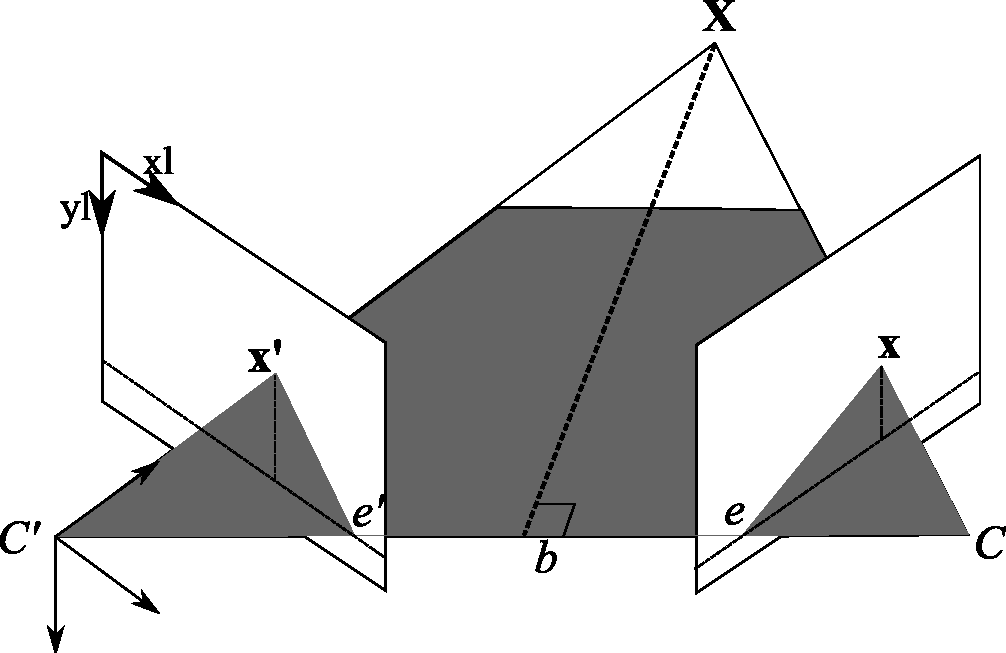
\includegraphics[width=0.8\textwidth]{pics/epipolar}
    \caption{The epipolar geometry}
    \label{chap2:fig-epipolarGeometry}
\end{figure}

This allows for the following facts which simplifies the computations a great deal.
\cite{epipolar}
\begin{itemize}
    \item Every 3D point in view of the cameras is constrained in an epipolar plane that
        intersects each image in an epipolar line.
    \item The \emph{epipolar constraint} says that a given feature in one image must lie
        along the corresponding epipolar line in the other view.
    \item The epipolar constraint means that the two-dimensional search for matching
        features simplifies to a one-dimensional search along the epipolar lines once the
        epipolar geometry of the stereo rig is known.
    \item The order is preserved. If two points are visible in both images and occur
        horizontally in that order in one image, they occur in the same order in the other
        image.
\end{itemize}

\paragraph{The Essential and Fundamental Matrices}
This matrices contains information about the translation and rotation which relate the
two cameras. The Essential matrix describes this translation and rotation in physical
space, while the Fundamental matrix also contains information about the intrinsics of the
two cameras, thereby describing the rotations and translations in pixel related
coordinates.

The derivation of the Essential matrix is interesting and is given here for reference.
Suppose a point $P$ related in the left camera coordinates, i.e. $P_l$ and the right
camera is located at $T$. The coordinates of $P_l$ in the right camera coordinates will
then be.
\begin{equation}
    \label{chap2:eq-Pr}
    P_r = R (P_l - T)
\end{equation}
Now, the epipolar plane is introduced. All points, $\mathbf{x}$ that lay on the plane with normal vector
$\mathbf{n}$ and passing through $\mathbf{a}$ obeys the equation,
\begin{equation*}
    (\mathbf{x} - \mathbf{a}) \cdot \mathbf{n} = 0
\end{equation*}
The cross product of $T$ and $P_l$ then becomes the normal vector of the epipolar plane,
because the epipolar plane includes both this vectors. Equation \eqref{chap2:eq-Pr} can be
rewritten as $P_l - T = R^{-1} P_r$ and including the cross product yields 
\begin{equation}
    (R^{-1} P_r)^T (T \times P_l) = 0
\end{equation}
The cross product can be expressed as a product between matrices by introducing the
skew-symmetric matrix $S$. \cite{modsim}
\begin{equation}
    S = \left [ \begin{array}{ccc}
                0 & -T_z & T_y \\
                T_z & 0 & -T_x \\
                -T_y & T_x & 0 \\ \end{array} \right]
\end{equation}
The essential matrix might now be defined with $R^{-1} = R^T$ and moving it behind $P_r$.
\begin{equation}
    E = RS 
\end{equation}
which gives the equation
\begin{equation}
    \label{chap2:eq-fundamental}
    P_r^T E P_l = 0
\end{equation}
$P_r$ and $P_l$ are the real world 3D coordinates, and can be transformed to 2D
coordinates by the perspective transformation derived by the pinhole camera model. 

The relation between the Essential matrix and the Fundamental matrix can be showed with
help of the camera intrinsic matrix $M$, because we know that $q = Mp$, where $q$ are
pixel coordinates and $p$ are the 2D world coordinates. Substituting for $P$ in Eqauation
\eqref{chap2:eq-fundamental} gives: \cite{openCV}
\begin{equation}
    q_r^T(M_r^{-1})^T E M_l^{-1} q_l = 0
\end{equation}
The definition of the fundamental matrix, $F$ is then
\begin{equation}
    F = (M_r^{-1})^T E M_l^{-1}
\end{equation}
Both matrices are $3\times3$ and have rank two with seven parameters.


\paragraph{Finding Stereo Correspondences}
Now that the mathematics which describes points in the different views to each other, the
case of matching the same points together can begin. This is obviously only possible for
visual areas that the two camera views overlap. 

There are couple of different matching algorithms. The most common are \emph{block
matching} algorithms. In \cite{konolige} a practical implementation of the block
matching algorithm are described. This algorithms use sum of absolute difference (SAD) windows to match same
same points in the two views. This algorithm work only on undistorted, rectified stereo
images. It first normalizes the image brightness which enhances textures. Then the search
for correspondences are carried out along the horizontal epipolar lines using the sum of
absolute difference window. After this the results are filtered to eliminate bad stereo
matches. This algorithm works best in highly textured environments, like outdoor
environments, and will prove less effective in structured surroundings like office
corridors and inside smooth pipelines. 

Another common matching algorithm are \emph{graph cut} algorithms. 

An extensive review of the different matching algorithms and their computational costs
can be seen in \cite{stereo-algorithms}.


\paragraph{Disparity and depth calculations}
When finally the stereo correspondences are found, the \emph{disparity} can be calculated.
The disparity is the difference in pixels coordinates from of the matched feature from one
image to the other. This disparity is inversely proportional to the depth. This means that
the depth perception of the stereo rig is better when relatively close to the cameras, as
Figure \ref{chap2:fig-disparity-depth} shows. 
Since the disparity is an integer, the resolution of the Stereo Rig depends on the
baseline. The figure shows the depth-disparity plot with 6 different baselines, $20,
60, 100, 150, 200$ and $300$ millimeters. It is clearly seen that the depth resolution becomes better
when the baseline increases. 
\begin{figure}[htbp]
    \centering
    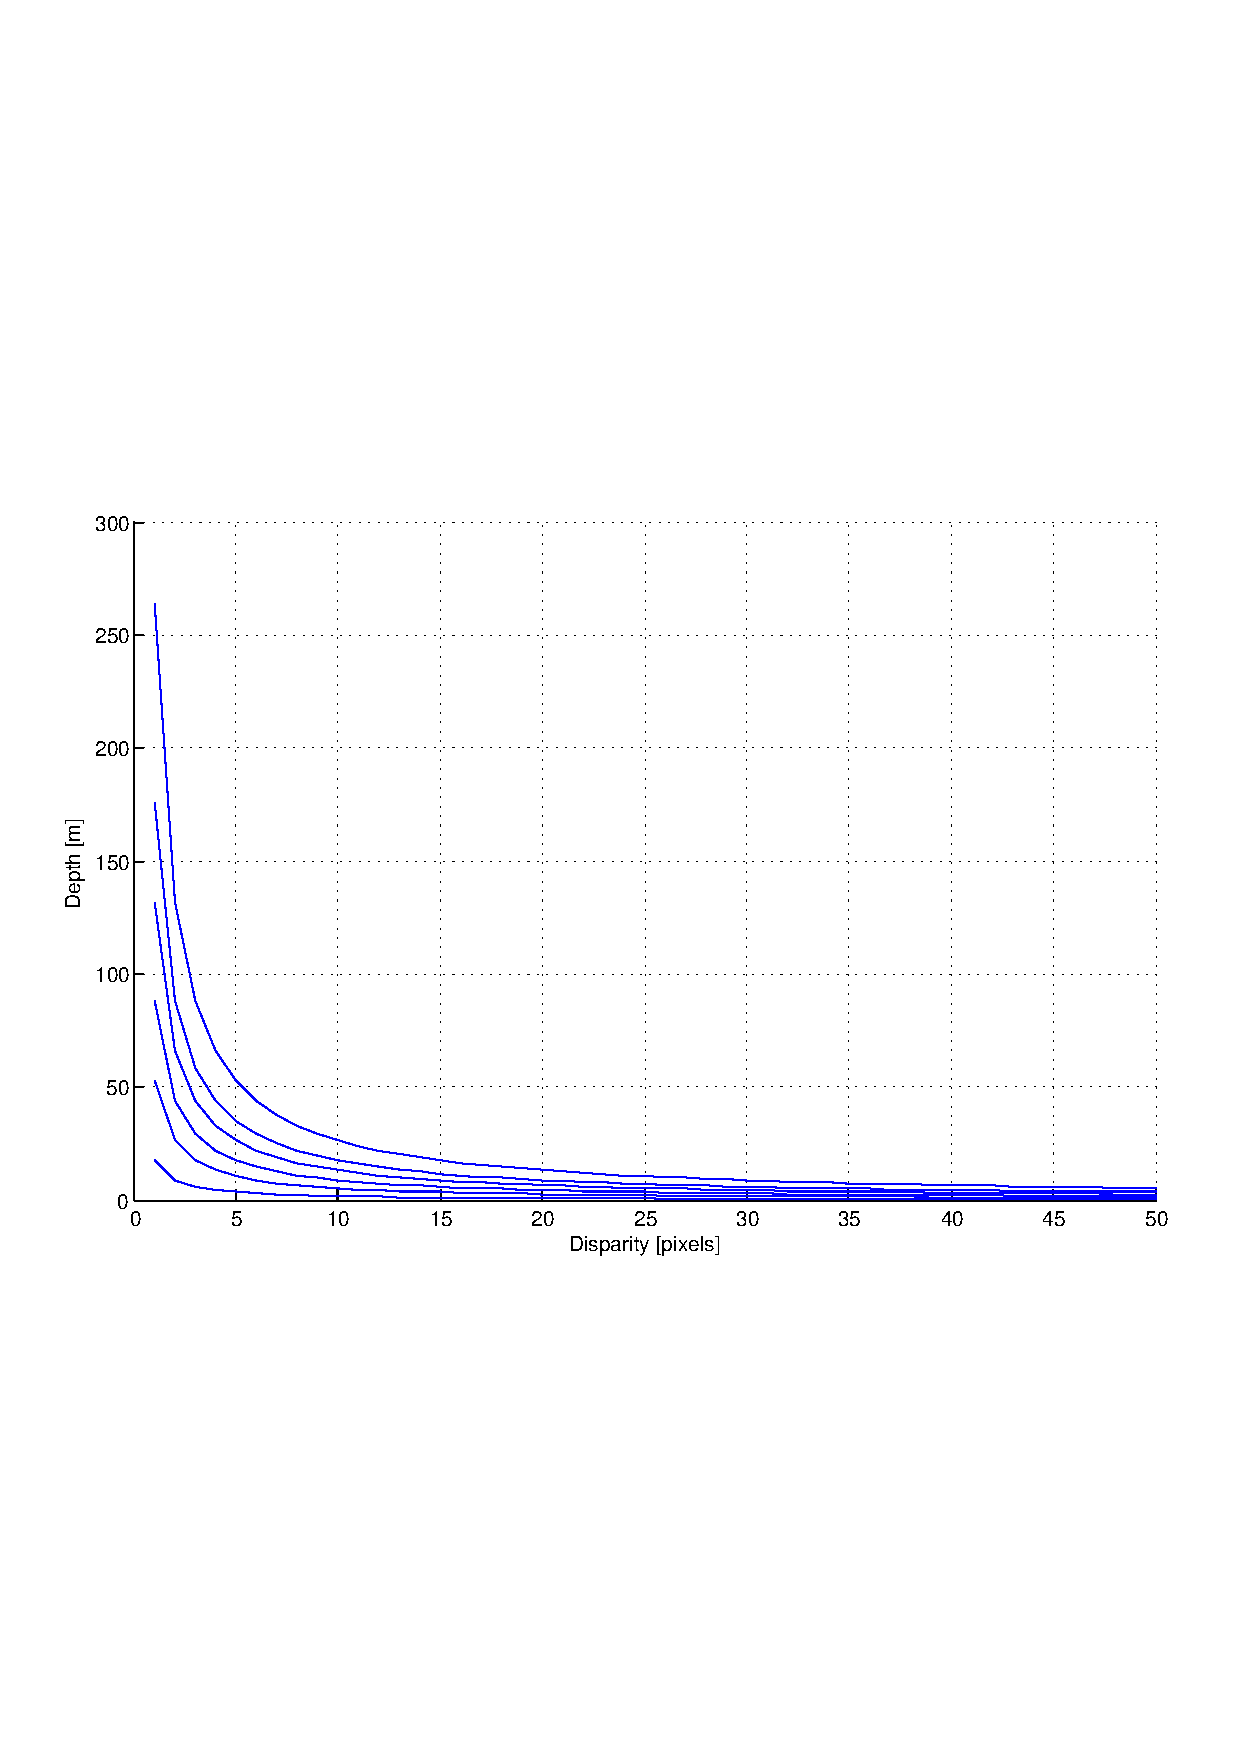
\includegraphics[width=0.7\textwidth]{pics/disparity}
    \caption{The relationship between depth and disparity}
    \label{chap2:fig-disparity-depth}
\end{figure}

Many robotic applications using stereo cameras utilizes the disparity maps directly,
because they usually just require the detection of obstacles. ****REFERENCES ON THIS****

The 3D coordinates of the point can be calculated form the disparities given by the
matching algorithms. This is the process of \emph{reprojection}. Using triangulation
between the two known camera locations the depth can be derived accordingly to 
\begin{equation}
    z = \frac{f T}{x_l - x_r}
\end{equation}

\subsubsection{Time-of-Flight Cameras}
The research and application of Time-of-Flight cameras have increased significantly during the last four
years. A Time-of-Flight camera is a compact device which makes it suitable to mount on
mobile platforms, and thereby using it in navigation and localization applications. 

The most used ranging techniques by the cameras are \emph{intensity modulation} approaches and
\emph{optical shutter} technology. The first one is used by the best known manufacturers,
like MESA and PMD. While the optical shutter approach is less expensive and have been used
by Zcam, which now have been sold to Microsoft. 


\paragraph{Intensity Modulation Approach}
\label{chap2:subsec-tof}
This approach uses modulated near infrared light (NIR), $g$ which is reflected to and
captured by a CCD chip then correlated with the reference signal, $r$. 
\begin{equation}
    c(\tau) = g \otimes r = \lim_{T \rightarrow \inf} \int^{T/2}_{-T/2} g(t) r(t + \tau) dt
\end{equation}
where the signals, $g$ and $r$ might be
\begin{equation}
    g(t) = \cos{\omega t}, \quad \quad r(t) = b + a \cos{(\omega t + \phi)}
\end{equation}
where $\phi$ is the phase offset because of the travel time of the signal, $b$ is a
correlation bias, $a$ is the amplitude and $\omega$ is the modulation frequency. Solving
the integral yields 
\begin{equation}
    c(\tau) = \frac{a}{2} \cos{(\omega \tau + \phi )} + b
\end{equation}
which is the correlation function. 

The demodulation is usually done by sampling the correlation function at 4 equally spaced
phase offsets. The following relation can now be written
\begin{equation}
    \begin{aligned}
        \phi &= \tan^{-1} (\frac{A_3 - A_1}{A_0 - A_2}) \\
        I &= \frac{A_0 + A_1 + A_2 + A_3}{4} \\
        a &= \frac{\sqrt{(A_3 - A_1)^2 + (A_0 - A_2)^2}}{2}
    \end{aligned}
\end{equation}
where $A_i = c(i \frac{\pi}{2})$ for $ i = 0,..,3$ and $I$ is the intensity of the returned NIR
signal. From this the distance can be calculated using the phase delay $\phi$. 
\begin{equation}
    d = \frac{c}{4 \pi \omega} \phi
\end{equation}

There are a number of challenges when using this approach
\cite{time-of-flight-comp-graphics}
\begin{itemize}
    \item The resolution of the sensors are small compared to standard RGB or grayscale
        sensors. Current resolution on present day time-of-flight cameras are $204 \times
        204$. 
    \item ``Wiggling'' because of imperfections when creating the sinusoidal signals.
    \item Errors due to intensity measurements. Various sensor electronics might influence
        the measured intensity and give wrong readings.
    \item ``Flying Pixels'' occurs when a pixel in the camera oversees a region with
        large depth variances, e.g. at object boundaries, because of superimposed signals. 
    \item Motion artifacts might occur because the phase images are captured sequentially
        quick motion might cause artifacts.
    \item Multiple reflections in highly reflective environments will cause erroneous
        distance measurements.
\end{itemize}

Standard lenses are used to capture the reflected light, which means that intrinsic
calibration should be carried out to specify the projection axis and distortion parameters
of the lens. See sections below for lens calibration and distortion coefficient
estimation. \cite{time-of-flight-comp-graphics}


\paragraph{Optical Shutter Approaches}
Light travels roughly at $c \approx 3 \times 10^8$ meters per seconds. This translates to
that light uses $7$ pico seconds to travel one millimeter. Imagine a light pulse emitted
at time $t$. This pulse travels in a spherical pattern and hits a 3D shape. The light wall
will be reflected back in a distorted pattern.\cite{optical-shutter} 
A shutter in front of the CCD chip then
shuts out the rest of the light wall pattern. This will then produce a shape of the object
which can be used to calculate the distance, based on the times the shutter is open,
according to the following relation \cite{time-of-flight-comp-graphics}
\begin{equation}
    d = (1 - \alpha) d_{min} + \alpha d_{max}, \quad \quad \alpha =
    \frac{I_{gate}}{I_{total}}
\end{equation}
where $I_{gate}$ is the pixel intensity which arrives when the shutter is open, and
$I_{total}$ is the total amount of reflected light. Distances outside $d_{min}$ and
$d_{max}$ cannot be measured in the exposure. Therefor this techniques require multiple
exposure to get the desired depth resolution. 

This method is also prone to the challenges stated for the intensity modulation approach
as well.

\paragraph{3D camera calibration}
Some of the uncertainty and difficulties described above can be attenuated by properly
calibrating the Time-of-Flight sensor. Since the sensor uses a conventional lens to
capture the returned light, distortion due to the lens might occur. This can be calibrated
using the same method as for normal cameras, described in Section
\ref{chap2:sec-distortion}. 

Depth inaccuracies are present because generation of a perfect sinusoidal signal which is
assumed for the correlation step is not possible due to cost and hardware limitation. This
is the base for a systematic distance error, which when analyzed have a sinusoidal shape
\cite{tof-calibration}. To correct this the systematic error function is approximated
using linear or higher-order polynomial models. 





\section{Map Data Representation}
\label{chap2:sec-representations}
The representation of sensor data is important for the functionality of the robot. This is
dependant on the amount of processing power and capacity that is available at the robot.
The area which the robot is to map is also of great importance when choosing the
representation. There are a number of representations that are tried out, and each one has its good and
bad abilities. 

The major representation methods which is used in literature are summarized in the below
sections. There are two major ideas when it comes to map representation, and that is
metric and topological.

Metric representation uses the sensor data as we see it. It is the direct Cartesian
representation of the way the world is. Examples of this are CAD drawings of floor plans
and housing. This maps are often large and inexact, because of many kinds of
uncertainties.

Topological representations uses a more abstract way. The world are represented by graphs,
which is nodes and links between them. This are a sparse and efficient way of representing
the world, but need more processing when the map is built. This kind of maps are not
exact, because they are not expected to be. They simply describe the connection between
different kind of objects, and all objects might have attributes describing how it really
looks. This method is useful in highly structured environments, such as pipelines, sewers,
and office landscapes. This because a series of junctions might tell you where you are
than just the metric information, which might be quite erroneous. 


\subsection{Occupancy Grid Maps}
Occupancy grid maps are a metric approach to the mapping problem and are widely used in 
robotic mapping, mostly because of it is simple to implement and use. It was developed 
by Elfes and Moravec in the mid 1980s, \cite{elfes}, \cite{moravec}. The method is quite 
robust and it is simple to implement with many kinds of sensors. This method assumes that 
the robots pose is known.

This method divides the world into grids with probabilities that the grid is occupied. It
starts with all grids at 50 \%, equal probability that the space is occupied or not. As
the robot moves around it updates the grids according to its sensor readings. When for
example employing laser range finders, the grid at the distance reported from the range
finder are marked as occupied according to some uncertainty set by the accuracy of the
range finder. The grids between the possible detected obstacle will then be decreased
because the probability of obstacles are less. 
\begin{figure}[htbp]
    \centering
    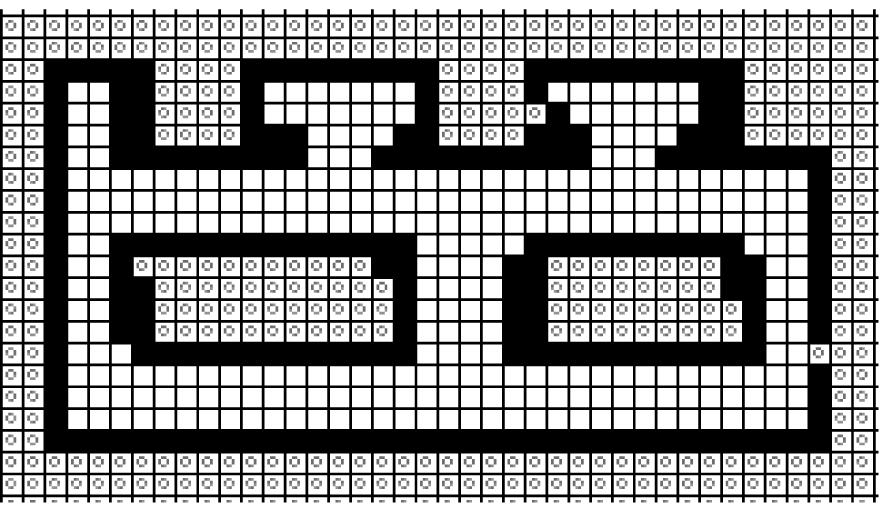
\includegraphics[width=0.7\textwidth]{pics/occupancy-grid}
    \caption{An example of the occupancy grid map}
    \label{chap2:fig-occupancy-grid}
\end{figure}

Occupancy maps are not the most computationally effective way to represent the world,
especially when it is big. It is cumbersome and may lead to problems when dealing with
cyclic environments. This because of the uncertainty in the sensor measurements and robots
pose and odometry. 


\subsection{Quad- and Oct-trees}
Quadtrees can be used to represent a 2D space by recursively dividing the space into
exactly four rectangles or squares. If this rectangles or squares does not include
interesting information then it will not be divided further. This dividing continues until
the smallest possible square is achieved. This creates a tree structure which is easily
traversed and searched if necessary. An \emph{Oct-tree} is the same only each node have
eight child nodes instead. This can be used to represent 3D spaces, see Figure
\ref{chap2:fig-octtree}.
\begin{figure}[htbp]
    \centering
   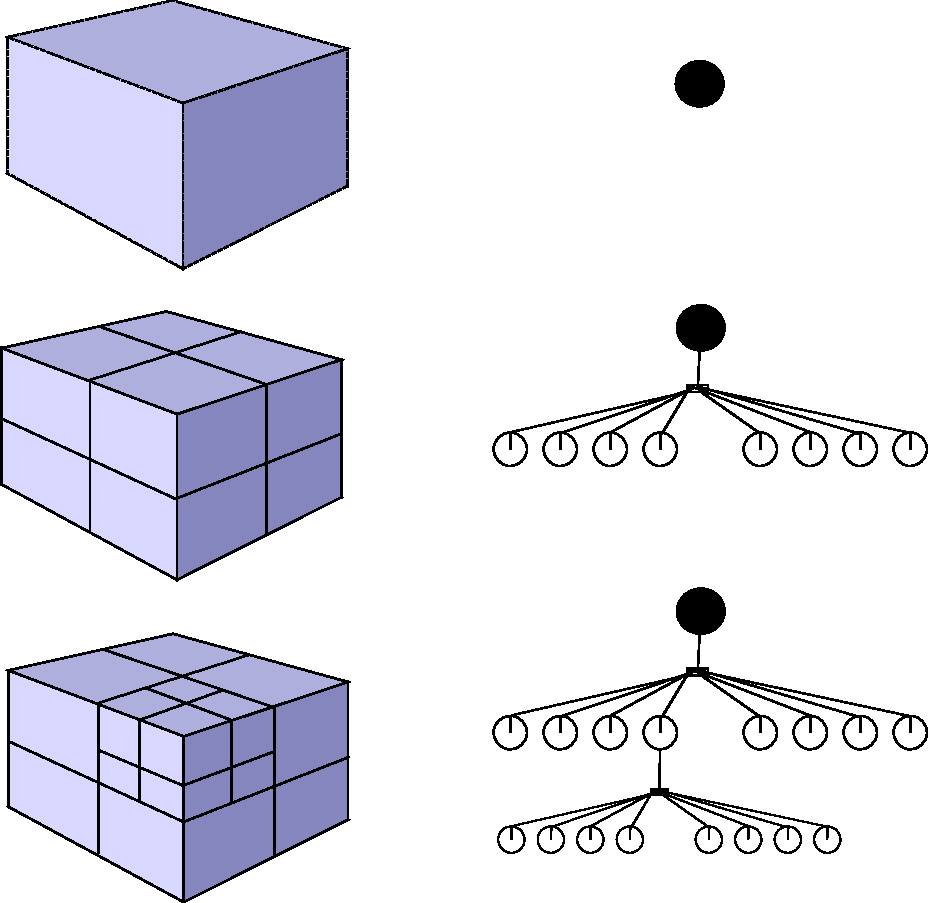
\includegraphics[width=0.5\textwidth]{pics/octtree}
    \caption{A Quadtree representation}
    \label{chap2:fig-octtree}
\end{figure}


\subsection{Topological Maps}
Object maps are topological maps and represents the sensed world in the form of predefined nodes and links
between them. Each node has a set of attributes, like length, links to doors etc. This is
a compact way to express the world and is much more computationally effective with larger
maps than the occupancy grid maps might be. Examples of such nodes are corridors,
junctions and dead ends, but this nodes must be suited to the application of the robot. 

The problem with this representation is that it needs a lot of input \'a priori. The
operator creates and inputs the map to the robot, which uses this map for navigation. The
largest challenge with this is to make the robot aware of where it is. It needs in some
way to recognize its surroundings, and match it to the \'a priori map.

The map of the London Underground is an common every day example of a topological map. It describes
the important things as stations, but not the geometrical distances which is not important
when navigating the London Underground. 


\subsection{Mixed Approaches}
This is when you take the best of both worlds. The easy and effective way of the metric
maps, and mix them with the abstract topological maps. This will help reduce the size of
the maps in the robots memory, and also make it more computationally effective because the
maps are sparse. 

******?????The mixed approaches are usually not computed on-line***???? (CHECK THIS). This utilizes
the metric approach for the rooms that have a lot of details, chairs, desks etc. and for
corridors and less detailed areas the topological approach, when the metric and
geographical information are not that important. 

This requires lots of processing of the sensor and map data, and should be done off-line
after the robot's mission is finished. 
\cite{thrun}

\section{Sensor Fusion Techniques}
Multi sensor fusion have been a target for much research. The topic seeks to combine the
abilities of several sensors and sensor types, to make the combined result better. 


According to \cite{sensor-fusion-mobile-robots} theres a lot of ways to achieve sensor
fusion in mobile robotics. The use of multiple sensors are favorable because the readings
can be fused to make a better estimate of the current situation. 

Multi sensor fusion are widely used in robotics today. This because it allows the designer
to use different measurement principles which have different capabilities. 


\begin{itemize}
    \item Low-level Fusion with unknown statistics
        \begin{itemize}
            \item Rule-based
            \item Geometric and topological maps
        \end{itemize}
    \item Low-level Fusion with known statistics in centralized approaches
        \begin{itemize}
            \item Kalman Filter and probabilistic approaches
        \end{itemize}
    \item Low-level fusion with known statistics in decentralized architectures
        \begin{itemize}
            \item Decentralized probabilistic approaches
        \end{itemize}
    \item High-level Fusion
        \begin{itemize}
            \item Behaviour-based architectures
        \end{itemize}
\end{itemize}


\subsection{Low-level Fusion}
The term low-level fusion is often used when the sensor data is directly integrated
resulting in parameters and state estimates of the model. This methods are mostly purely
mathematical. This method involves the Kalman Filter, and other Bayesian approaches. In
many cases the use of \'a priori information are utilized to verify or improve the
estimates from the sensors.

This methods are probabilistic and requires that you know something about the
statistical properties of the sensors and the \'a priori model. 


\subsection{High-level Fusion}



\subsection{Interpolation Techniques}



\subsection{Probabilistic Techniques}



\section{Feature Extraction}
\label{chap2:sec-feature-extraction}
The need for feature extraction should be obvious when dealing with autonomous robot
navigation. For the robot to know where it is it needs to recognize its surroundings. This
is a difficult step, because computers are not known to be very good at this, as the human
brain is. 

By feature extraction it is meant to recognize one point or feature in one instant and
find the same point at the next time instant. This can be imagined difficult in some
surroundings where theres little individual detail. 

This problem is relaxed a bit when the surroundings are confined to pipelines. The problem
here is that the interior of the pipeline are not rich in detail, and is mostly the same
everywhere the robot travels, except in the different kinds of junctions. By feature
extraction in this report the meaning is to recognize the different types of junctions
that the robot will travel through. 


\subsection{Point Feature Histograms}
Point feature histograms is a way of assessing the local geometry around a point in a
3D point cloud. This can be used to segment the point cloud into given geometrical
primitives. The computation of a point feature histogram works as follows, for each point
$p$, all of $p$'s neighbours inside a sphere with radius $r$ is selected. For every pair
of points in the selected subset the normals $n_i$ and $n_j$ are estimated. A Darboux
$uvn$ frame are defined according to 
\begin{equation}
    u = n_i, \quad v = (p_j - p_i)\times u, \quad w = u \times v
\end{equation}
The following angular variations are then used for categorizing the points. \cite{pfh}
\begin{equation}
    \begin{aligned}
        \alpha &= v \cdot n_j \\
        \phi &= (u \cdot (p_j - p_i)) / || p_j - p_i|| \\
        \theta &= \arctan (w \cdot n_j, u \cdot n_j)
    \end{aligned}
\end{equation}
These angular variations are sorted into histogram bins according to 
\begin{equation}
    idx = \sum_{i=0}^{i \leq 2} \left [ \frac{f_i \cdot d}{f_{i_{max}} - f_{i_{min}}}
    \right] \cdot d^i
\end{equation}
where $idx$ is the point feature histogram bin index, $d$ is the number of subdivision of
the features maximum theoretical value range $(f_{i_{max}} - f_{i_{min}})$. This will sort
the points into bins according to how the angular variations vary. 

Different geometric surface primitives have different signatures. \cite{pfh-geometric}
shows the distinct histogram formation for convex surfaces as cones, spheres, cylinders
and planes. This can be used to classify points and thereby isolating important features
in the scene. 

\cite{pfh-segmenting} uses a combination of local fast point feature histograms to segment
the object of interests into geometric primitives, then a global version of the point
feature histogram are employed to detect and categorize objects in the given scene. The
shown results are promising. 


\subsection{Surface Fit Algorithms}
\label{chap2:sec-surface-fit-alg}
Suppose a point on a 3D surface can be expressed as
\begin{equation}
    \mathbf{x} = f(\mathbf{s}, t)
\end{equation}
$\mathbf{s}$ is a parameter of size $p$ characterizing the nature of the surface, i.e. the
radius of a circle. $t$ is the positional parameters which fixes the position of the point
on the surface. For a sphere, the parameters vector, $\mathbf{s}$ would have four parameters,
the three dimensional position and the radius, while the $t$-vector would have 2
parameters representing the angles around two of the axes, in this case the spherical
coordinates.

The surface fit problem can be sated as a least-squares minimization problem. The
objective function to be minimized is then the distance form the data set to a cylinder
surface. The distance can be given as 
\begin{equation}
    d( \mathbf{s}, \mathbf{p})  = | ( \mathbf{p} - (\sigma + \frac{1}{k} \mathbf{n})
    \times \mathbf{a})| - \frac{1}{k}
\end{equation}
$\mathbf{p}$ is an arbitrary point, $\sigma \mathbf{n}$ is the point which is the closest
point on the cylinder to the origin, $\frac{1}{k}$ is the radius of the cylinder, and $\mathbf{a}$ is the
direction vector of the cylinder. $\mathbf{n}$ obeys the relation $\mathbf{a} \cdot
\mathbf{n} = 0$. 

\cite{ls-fit-cylinder} proposes to use an approximation to the distance, both because it
simplifies and the computational difficulties because of the square root vanishes, but
also to avoid computational singularities when calculating the distance. The proposed
expression to be minimized then becomes
\begin{equation}
    \tilde{d} = \frac{k}{2} |\hat{\mathbf{p}} \times \mathbf{a} | ^2 - \hat{\mathbf{p}} \cdot
    \mathbf{n}
\end{equation}
where $\hat{\mathbf{p}} = \mathbf{p} - \sigma \mathbf{n}$. This distance is robust to
mathematical singularities and is less computationally intensive than taking the square
root of something. The function which is to be minimized then becomes
\begin{equation}
    \label{chap2:eq-ls-cylinder-min}
    \sum_i \tilde{d}^2(\mathbf{s}, \mathbf{p}_i)
\end{equation}
The cylinder can be completely described and parametrized with the \emph{direction cosines} the radius, and
the position of the axis. The various minimization algorithms can be used and will be
discussed in the next section.


\subsubsection{Leasts-Squares Gauss-Newton Optimization}
\label{chap2:subsec-gauss-newton}
Least-squares method is a common way to optimize and fit data sets to a proposed model.
The idea is to minimize the objective function 
\begin{equation}
    f(x) = \frac{1}{2} \sum_{j = 1}^m r^2_j (x)
\end{equation}
where the $r_j(x) \in \mathbb{R}^n \rightarrow \mathbb{R}$ is called the \emph{residual} and
is generally a linear or nonlinear function. This function can be written as a vector then
the Jacobian can be defined as
\begin{equation}
    J (x) = \left[ \frac{\partial r_j}{\partial x_i} \right]
\end{equation}
The Jacobian is a $m \times n$-matrix. Using this the Hessian, i.e. the second order
derivative of $f$ can be expressed as
\begin{align}
    \nabla f(x) &= \sum_{j = 1}^m r_j(x) \nabla r_j(x) = J(x)^T r(x) \\
    \nabla^2 f(x) &= \sum_{j=1}^m \nabla r_j (x) \nabla r_j(x)Å T + \sum_{j=0}^m r_j(x)
    \nabla^2 r_j(x) = J(x)^T J(x) + \sum_{j= 0}^m r_j(x) \nabla^2 r_j(x)
    \label{chap2:eq-hessian}
\end{align}
This allows for that the Hessian, which usually is very cumbersome and computationally
intensive to calculate can be approximated by the Jacobian. This is especially true when
the residual terms are small.

The Gauss-Newton method uses is a modified Newton method that uses line search to find the
best fit. Standard Newton methods are based on solving $\nabla^2 f(x_k) p = -\nabla
f(x_k)$ with regard to $p$ to find the search direction. The Gauss-Newton approach uses
the approximation $\nabla^2 f_k \approx  J_k^T J_k$, which gives the following equation to
solve
\begin{equation}
    J_k^T J_k p_k = - J_k^T r_k
\end{equation}
The approximation of the Hessian saves quite a lot computational time and the impact on
the direction is not that great. Also, around the solution $x^*$ the first term in
\eqref{chap2:eq-hessian} will dominate the other factors. This will cause the convergence
rate of the algorithm to be equal to those of the standard Newton methods, which is
quadratically.\cite{optreg} 

$p_k$ is guaranteed to be a descent direction when $J_k$ has full row rank and the
gradient $\nabla f_k$ is nonzero. The Gauss-Newton also has the advantage that the
nonlinear objective function might be divided into linear subproblems and solved
individually. This means that the search direction, $p_k$ is the solution of
\begin{equation}
    \min{p} \frac{1}{2} || J_k p + r_k ||^2
\end{equation}

The term which is minimized is \eqref{chap2:eq-ls-cylinder-min} subject to the direction
of the cylinder axis, the radius and the start position center of the axis. 


\subsubsection{RANSAC Algorithm}
Standard fitting techniques uses the whole dataset when fitting a function to it. This
means that it assumes that errors and ``wild points'' in the dataset can be averaged out.
Said in another way, the correctness of the dataset is a function of the size of the
dataset. When for example in computer vision, graphical primitives such as planes, and
cylinders are in the same scene, it is difficult to know which points in the dataset
correspond to which graphical primitive. Therefor, one will need to sort out which points
``belong'' to the different primitives. If a least-squares approach is used the fitting
procedure to the primitives would not be very successful because this method will assume
that all points have some relation to the fitted primitive. \cite{ransac}

RANSAC is an acronym of \emph{RANdom Sample And Concensus}. This algorithm is a
non-deterministic algorithm which is robust to ``wild points'' in the dataset. This is
practical when the datasets are polluted with noise and measurements errors.
The RANSAC algorithm is basically a two step process, which is repeated until some
criterion is fulfilled. The first step is called the \emph{hypothesize}-step which selects
the \emph{minimal sample set} (MSS). This is the absolute minimum required to represent
the fitted model, i.e. for a 2D line, two points are needed to uniquely define the
line. The model parameters are computed using only the points from the MSS.

The next step is the \emph{test}-step, which determines the amount of points from the
whole dataset which are consistent with the parameters computed form the MSS set. This set
of points are called the \emph{consensus set} (CS). The algorithms search for points
terminates when the probability of generating a better consensus set drops below a certain threshold, i.e.
more points can be added to the consensus set. The distance from the points in CS to the 
fitted model is used as a measure on how good the model is. This model is kept as the best
fit up to date. \cite{ransac-dummies}

This is done a finite number of times and dependant on the number of \emph{inliers}, i.e.
a point that are defined to belong to the model, the model is compared to the present best
fit or rejected.

To ensure that RANSAC gives the best fit model, the number of iterations to find the best
fit must be large enough. Since the selection of the initial MSS is done randomly, one
cannot guarantee that the MSS only consists of inlier points. The probability of
selecting $h$ sets which are polluted by \emph{outliers} is $(1 - q)^h$, where $q$ is the
number of inliers in the dataset. The idea is to pick a $h$ large enough that the
probability that all the sets are contaminated by outliers will be lower than a certain
value, $\epsilon$ called the \emph{alarm rate}, $(1 - q)^h \leq \epsilon$. Reorganizing
this to find the number of iterations
\begin{equation}
    \hat{T}_{iter} = \left \lceil \frac{\log \epsilon}{\log (1 - q)} \right\rceil
\end{equation}
In general the number $q$ is difficult to calculate, according to \cite{ransac-dummies}
the probability can be approximated by 
\begin{equation}
    q = \prod_{i = 0}^{k-1} \frac{N_I - i}{N - i} \approx \left ( \frac{N_i}{N} \right)^k
\end{equation}
where $N_I$ is the total number of inilers, $N$ is the total number of points in the
dataset, and $k$ is the number of times one will try to pick a set of inliers. This can be
approximated because $k$ most probably are much much smaller than both $N$ and $N_I$. A
estimate of the number of inliers can be found, using the number of inliers found
up-to-date. \cite{ransac-dummies}


\subsubsection{M-SAC Criterion}



\section{State-of-the-Art Pipe Inspection Robots}
\label{chap2:sec-state-of-the-art}
The German MAKRO project \cite{MAKRO-project} uses a multi-segmented robot, each segment 
having three degrees of freedom, panning, tilting and rotation. This is a complete
research project to create a fully autonomous sewer inspection robot. The robot is
equipped with various sensors including, a stereo camera rig for dense stereo
reconstruction of the pipe structure. Proximity IR sensors directed perpendicular to the
motion axis to sense the pipe walls, and an ultrasound sensor directed forward for
position measurements. An experimental set-up with a laser to project a predetermined
pattern on the surroundings together with one of the cameras to calculate the direction of
th sewer pipe axis. The control system is based on an AI machine learning method called \emph{Q-Learning}, in
a closed-loop, hierarchical fashion.


\cite{MRINSPECT-V} proposes a method of visual landmark recognition by using shadows
generated by a special illuminator. The method where implemented on \emph{MRINSPECT V}, a
four-segmented robot, where two modules are driving modules with four wheels presented at
120 degrees interval around the module, one at the front and one at the end. The two
remaining modules contains the batteries and control modules. 
The captured images form a camera is filtered and the
shadows are extracted using a binarization and thresholding. The shadow profiles are
labeled with unique ID-tags and the center of the shadow are calculated. Depending on
where the shadows are cast, the direction of the pipe feature can be determined. The
shadow pattern are matched against a database to determine what kind of profile the robot
are going trough. The shadow detection system is used to locate profiles and term them as
landmarks. When the robot are going through the landmark, a 2-axis gyro and otometry of
the wheels are used to determine the direction and length of the landmark and updating
this to the internal landmark database. When the robot have passed the landmark, the 
landmark search using shadows are restarted. This method were tested on a 8 inch (20 cm)
gas-pipeline structure, with L-shaped and T-shaped junctions arranged in a 3D dimensional
arrangement and showed promising results. 


\emph{Kario-II} is a multi-segmented robot, typically made up of 6 drive segments with
active wheels and 5 joints between these segments which each have 3 degrees of freedom,
making a total of 21 degrees of freedom of the robot. \cite{Kairo-II} provides a control
strategy of controlling and path planning for the full 21 DOF model in unstructured and
dynamic environments.******* 


\cite{KANTARO} describes \emph{KANTARO}, a single segement, sewer-pipe inspection robot 
capable of moving autonomously in 200-300 mm pipes. The robot turns smoothly in 90 degrees 
junctions and able to go down 5 cm steps. The robot consists of a platform of 4 wheels,
and a payload box placed on top. The robot is equipped with a CCD camera with ``fish eye''
lens and proper lighting together with a laser scanner. This laser scanner is custom made
for and uses the optical triangulation principle and produces measurements with accuracy
of about 1 mm. KANTARO have been tested in a dry sewer test environment, traversing
L-bends, T-junctions with high stability, according to the authors. But much work is still
to be done with regard to make this robot robust enough for the real world. 

\cite{KURT}


\cite{sintef-tof} uses a Time-of-flight camera mounted on the Pipe Inspection Konda. It
uses the M-SAC criterion to fit a cylinder or a cone to the sensor output of the
time-of-flight camera. The cone was used instead, because experiments showed that it gave
a better fit to the dataset. The system then uses the difference between the fitted
cylinder or cone and
a ideally synthesized image of the scene to find junctions and other things worth noting.
The system is implemented with obstacle avoidance and gives promising results. This report
is loosely based on the method described in the article. 


